\documentclass[]{article}
\usepackage{lmodern}
\usepackage{amssymb,amsmath}
\usepackage{ifxetex,ifluatex}
\usepackage{fixltx2e} % provides \textsubscript
\ifnum 0\ifxetex 1\fi\ifluatex 1\fi=0 % if pdftex
  \usepackage[T1]{fontenc}
  \usepackage[utf8]{inputenc}
\else % if luatex or xelatex
  \ifxetex
    \usepackage{mathspec}
  \else
    \usepackage{fontspec}
  \fi
  \defaultfontfeatures{Ligatures=TeX,Scale=MatchLowercase}
\fi
% use upquote if available, for straight quotes in verbatim environments
\IfFileExists{upquote.sty}{\usepackage{upquote}}{}
% use microtype if available
\IfFileExists{microtype.sty}{%
\usepackage{microtype}
\UseMicrotypeSet[protrusion]{basicmath} % disable protrusion for tt fonts
}{}
\usepackage[margin=1in]{geometry}
\usepackage{hyperref}
\hypersetup{unicode=true,
            pdftitle={Project 1 Redwood Data Report},
            pdfauthor={Phoebe Abramowitz(26386343) \& Omri Newman(3032273024)},
            pdfborder={0 0 0},
            breaklinks=true}
\urlstyle{same}  % don't use monospace font for urls
\usepackage{graphicx,grffile}
\makeatletter
\def\maxwidth{\ifdim\Gin@nat@width>\linewidth\linewidth\else\Gin@nat@width\fi}
\def\maxheight{\ifdim\Gin@nat@height>\textheight\textheight\else\Gin@nat@height\fi}
\makeatother
% Scale images if necessary, so that they will not overflow the page
% margins by default, and it is still possible to overwrite the defaults
% using explicit options in \includegraphics[width, height, ...]{}
\setkeys{Gin}{width=\maxwidth,height=\maxheight,keepaspectratio}
\IfFileExists{parskip.sty}{%
\usepackage{parskip}
}{% else
\setlength{\parindent}{0pt}
\setlength{\parskip}{6pt plus 2pt minus 1pt}
}
\setlength{\emergencystretch}{3em}  % prevent overfull lines
\providecommand{\tightlist}{%
  \setlength{\itemsep}{0pt}\setlength{\parskip}{0pt}}
\setcounter{secnumdepth}{0}
% Redefines (sub)paragraphs to behave more like sections
\ifx\paragraph\undefined\else
\let\oldparagraph\paragraph
\renewcommand{\paragraph}[1]{\oldparagraph{#1}\mbox{}}
\fi
\ifx\subparagraph\undefined\else
\let\oldsubparagraph\subparagraph
\renewcommand{\subparagraph}[1]{\oldsubparagraph{#1}\mbox{}}
\fi

%%% Use protect on footnotes to avoid problems with footnotes in titles
\let\rmarkdownfootnote\footnote%
\def\footnote{\protect\rmarkdownfootnote}

%%% Change title format to be more compact
\usepackage{titling}

% Create subtitle command for use in maketitle
\newcommand{\subtitle}[1]{
  \posttitle{
    \begin{center}\large#1\end{center}
    }
}

\setlength{\droptitle}{-2em}

  \title{Project 1 Redwood Data Report}
    \pretitle{\vspace{\droptitle}\centering\huge}
  \posttitle{\par}
    \author{Phoebe Abramowitz(26386343) \& Omri Newman(3032273024)}
    \preauthor{\centering\large\emph}
  \postauthor{\par}
      \predate{\centering\large\emph}
  \postdate{\par}
    \date{3/8/2019}


\begin{document}
\maketitle

\section{Paper Summary (20 pts)}\label{paper-summary-20-pts}

This study of microclimatic monitoring aims to get a better
understanding of the life of a Redwood tree in Sonoma, CA. To do this,
an interdisciplinary team from the University of California, Berkeley
designed an experiment that paints a picture of a redwood tree's
ecophysiology spanning fourty-four days in Spring 2004. They did this
using a unique network of nodes and wireless sensors to gather
spatio-temporal and environmental dynamic data over the entire organism.
Each of the thirty-three nodes collected hundreds of thousands of data
points, which lie in four different three-dimensional spaces (time x
height x value). This wireless sensor network, or macroscope, allows for
rich analysis on an unprecedented dataset.\\
After brainstorming with several biologists, Sonoma's coastal redwood
forest was chosen as the site of this study because of its dynamic
ecosystem. Longer daylight hours during the Spring provided sufficient
time for the photosynthetically active radiation sensors to collect
data, and the coastal fog coming off the Pacific guaranteed a wide range
of temperature and humidity gradients.\\
A thorough analysis of the redwood data confirmed the biologists'
hypothesis, which premised the existence of dynamic gradients present in
the redwood trees ecophysiology. By projecting the data points onto a
subset of the three-dimensions, the analysis task became simpler.\\
One drawback to using the sensor network was the presence of missing
values throughout the data set in both time and height dimensions.
However, the team worked in spite of this by studying distributions in
most of their analyses. In addition to confirming the team's hypothesis,
more information about the climatic distribution of the tree was
extracted from the analysis. One impactful step was using the data to
build a quantitative model of the effect of microclimatic gradients on
the sap flow rate of redwood trees. By better understanding this
process, biologists can piece together a more detailed picture of the
larger scale carbon and water exchange within a forest ecosystem.\\
The main variables of interest in this study are those that shed light
on the microclimate and ecophysiology of the redwood tree. Thus, each
data point can be viewed in three dimensions-- time, height, and value.
The values, recorded by the network of sensors, are temperature,
humidity, incident photosynthetically active solar radiation (PAR), and
reflected PAR. Collecting this data over an extended period of time
required a powerful system and precise deployment methodology. The data
collection time period started in late April and spanned fourty-four
days, sampling all sensors every five minutes. The nodes were placed
along the seventy meter redwood tree starting at a height of fifteen
meters, with two-meter spacing between nodes. The west side of the tree
had a thicker canopy that served as protection against environmental
effects, so the majority of the nodes were placed there. Lastly, the
nodes were placed close to the trunk (0.1-1.0 meter) such that the
recordings were of the microclimatic trends of the tree and not the
wider climate.\\
Multiple sensors were integrated into the Mica2Dot wireless node, as a
means to gather data on the environmental dynamics of the tree. This
node has a one inch diameter form factor, an Atmel microcontroller
running at 4 MHz, a 433 MHz radio from Chipcon operating at 40Kbps, and
512kB of flash memory. The node was packaged into a sealed cylindrical
enclosure made from white high-density polyethylene that reflects
radiated heat. The enclosure contained the node, battery, and two sensor
boards - one for direct radiation and one for all other measurements.
Data collected from these nodes were stored in a local database or
gateway, then transmitted to an offsite database via a general packet
radio service (GPRS) cellular modem. The UCB team used TASK software as
the node operating system and data collection scheme to aid with this
work. This multi-hop system utilized TinyOS and MintRoute systems to
retrieve data from the nodes and store them in the gateway as
efficiently as possible. The entire network of nodes was awake for four
seconds every five minutes, in order to take sensor readings, transfer
the data to the base stations, and then return to sleep.\\
Two calibration schemes were completed by the team to ensure a
satisfactory operation prior to setting up the final system. The first
calibration consisted of leaving the sensors on a roof collecting PAR
data every thirty second for two weeks to verify the accuracy of the
readings. The purpose of the second calibration was to understand the
response of the temperature and humidity sensors. The nodes were tested
in a controllable weather chamber that had varying temperature and
humidity conditions, and recorded readings every thirty seconds. The
calibration techniques used on the nodes took up space on the 512kB
flash memory. Thus, some of the data loggers in the local database
gateway ran out of memory before the end of the data collection time
period. These loggers were meant to serve as a backup in case of network
failure, and stored data in the case of lost GPRS connectivity. On the
other hand, the logger data that was stored in the gateway could only be
accessed at the end of the data collection time period, and there was
lost information in the nodes that ran out of flash memory. This defines
the main difference between sonoma-data-net.csv and sonoma-data-log.csv,
which both contain values the other is missing.

\begin{center}\rule{0.5\linewidth}{\linethickness}\end{center}

\section{\{Data cleaning (40 pts)\}}\label{data-cleaning-40-pts}

This data set contains gross outliers, inconsistencies, and lots of
missing values. We use basic exploratory data analysis and data cleaning
techniques to get a better understanding of the data, determine which
values make sense in the context of the study, and remove missing values
when necessary.

\begin{enumerate}
\def\labelenumi{\arabic{enumi}.}
\tightlist
\item
  For the initial comparison in hamatop (Incident PAR) between
  \textbf{sonoma-data-log.csv} and \textbf{sonoma-data-net.csv}, we
  remove outliers that are ten times larger than the third quartile in
  an effort to explore the ranges more thoroughly. We notice a slight
  bump in the right tail of incident PARs histogram for
  \textbf{sonoma-data-net.csv}, which does not occur in
  \textbf{sonoma-data-log.csv}.
\end{enumerate}

\begin{center}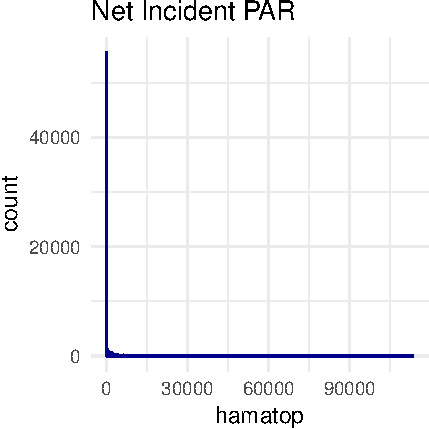
\includegraphics{Project1WriteUp_files/figure-latex/unnamed-chunk-2-1} \end{center}

\begin{center}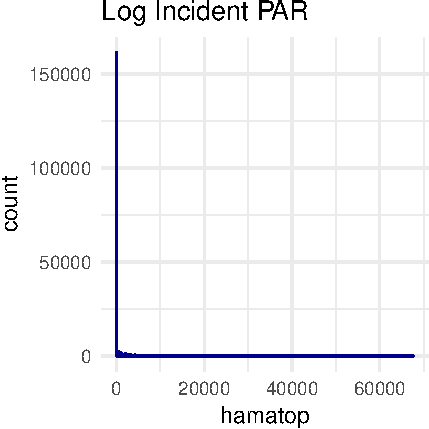
\includegraphics{Project1WriteUp_files/figure-latex/unnamed-chunk-2-2} \end{center}

The histograms for hamabot (Reflected PAR) reveal some interesting
trends shared by *** sonoma-data-log.csv** and
\textbf{sonoma-data-net.csv}. Not only are their ranges the same, but
they both exhibit the same gaps in the values of hamabot that occur.

\begin{center}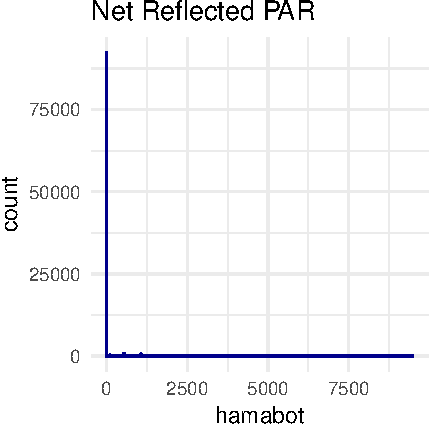
\includegraphics{Project1WriteUp_files/figure-latex/unnamed-chunk-3-1} \end{center}

\begin{center}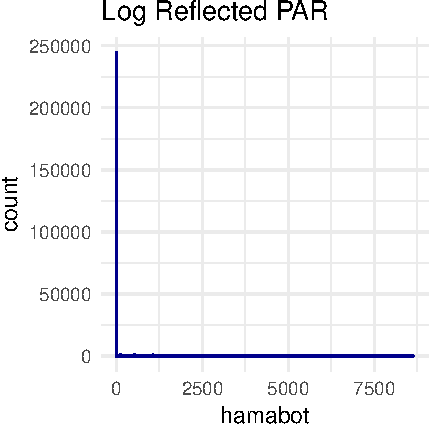
\includegraphics{Project1WriteUp_files/figure-latex/unnamed-chunk-3-2} \end{center}

It is clear from the histograms below that voltage readings are not
consistent between \textbf{sonoma-data-log.csv} and
\textbf{sonoma-data-net.csv}

\begin{center}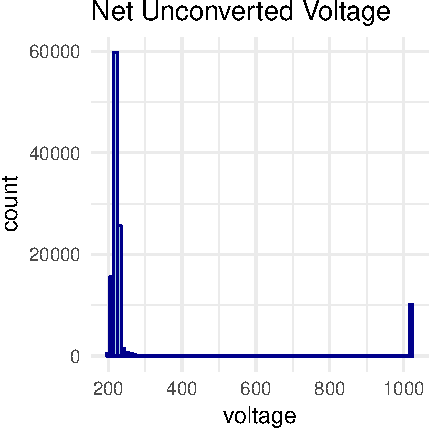
\includegraphics{Project1WriteUp_files/figure-latex/unnamed-chunk-4-1} \end{center}

\begin{center}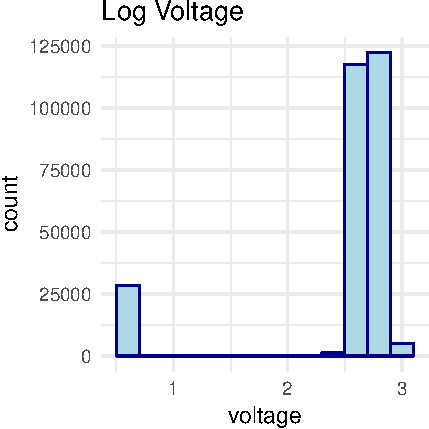
\includegraphics{Project1WriteUp_files/figure-latex/unnamed-chunk-4-2} \end{center}

To reconcile the inconsistencies between voltage and PAR, we applied two
separate conversions as to match the ranges from the paper:\\
The voltage readings in \textbf{sonoma-data-log.csv} are generally
within the correct range of just a few volts, while the readings in
\textbf{sonoma-data-net.csv} had significantly higher values. This
discrepancy can be attributed to the analog-to-digital converter used
within the ATmega128 node\textsuperscript{1}. To switch from the 10-bit
ADC readings to actual voltage measured, we followed a simple
ratiometric conversion scheme \textsuperscript{2}. We multiplied the
values by 12.33 and divided by 1023 to transform the data into the
desired range.

We also noticed the ranges for hamatop and hamabot differ from the
paper. We convert the measurements of both types of PAR from Lux to
PPMG, the units expressed in the visualizations in the study, using a
0.0185 conversion factor.

We then combine data sets from the log and the network into one main
data set. We take the values from the network dataset in cases of dual
instances, as the times are more precise.

In our main data table, we remove 3686 rows where the temperature,
humidity, reflective PAR, and incident PAR are missing. There are 3686
values missing for each of the 4 variables.

After removing missing data, reconciling inconsistencies, and joining
the \textbf{sonoma-data-log.csv} and \textbf{sonoma-data-net.csv}, we
incorporate the \textbf{mote-location-data.txt} using nodeid as a unique
identifier for each sensor. All together we have the location of each
mote, along with the respective sensor data. We selected only the
variables of interest amongst the 11 to create a desired dataset of all
the readings. Our main table has 337,744 observations and 12 variables.

After removing missing data, reconciling inconsistencies, and joining
the \textbf{sonoma-data-log.csv} and \textbf{sonoma-data-net.csv}, we
incorporate the \textbf{mote-location-data.txt} using nodeid as a unique
identifier for each sensor. All together we have the location of each
mote within the two trees, along with the respective sensor data. We
selected only the variables of interest amongst the 11 to create a
desired dataset of all the readings. Our main table has 337,744
observations and 12 variables.

We chose to match the range of each variable as they are presented in
the paper. It is clear in the following histograms that all of the
variables contain some outliers. Instead of removing these data points
per variable, we noticed that filtering out rows with faulty voltage
readings--which are not reliable, as detailed in the paper-- does the
same job in one fell swoop. Just as is described in the paper, filtering
out readings below 2.4V or above 3V removes 33,833 observations.

\begin{center}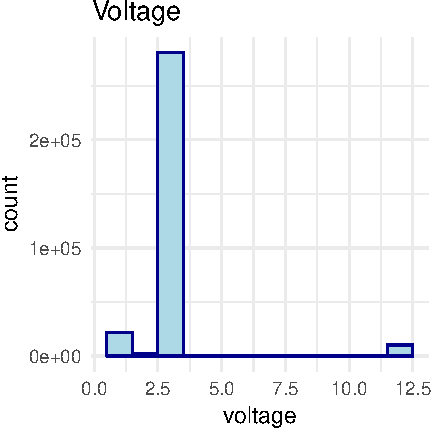
\includegraphics{Project1WriteUp_files/figure-latex/unnamed-chunk-9-1} \end{center}

\begin{center}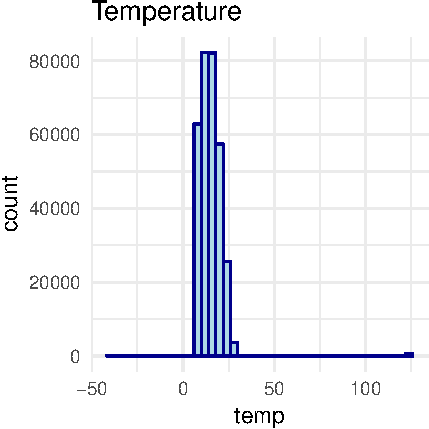
\includegraphics{Project1WriteUp_files/figure-latex/unnamed-chunk-9-2} \end{center}

\begin{center}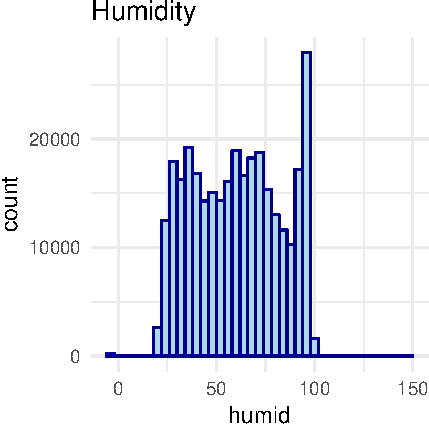
\includegraphics{Project1WriteUp_files/figure-latex/unnamed-chunk-9-3} \end{center}

\subsubsection{(Bonus) Discuss other possible outliers and explain your
reason why it is better to remove them than to keep
them.}\label{bonus-discuss-other-possible-outliers-and-explain-your-reason-why-it-is-better-to-remove-them-than-to-keep-them.}

\section{\{Data Exploration (40 pts)\}}\label{data-exploration-40-pts}

\begin{itemize}
\tightlist
\item
  We choose the subset of the data occuring during the week of May 23rd
  through May 30th. There are more hours of sunlight in the last week of
  May as the summer solstice gets closer. This subset--containing
  \textasciitilde{}28,000 values-- in particular has fewer missing
  values than other time periods, as shown in the histogram.
\end{itemize}

\begin{center}\includegraphics{Project1WriteUp_files/figure-latex/unnamed-chunk-10-1} \end{center}

\subsubsection{Some pairwise scatterplots of some variables and
descriptions of our
findings:}\label{some-pairwise-scatterplots-of-some-variables-and-descriptions-of-our-findings}

The number of the nodeid is not meaningfully correlated to height

\begin{center}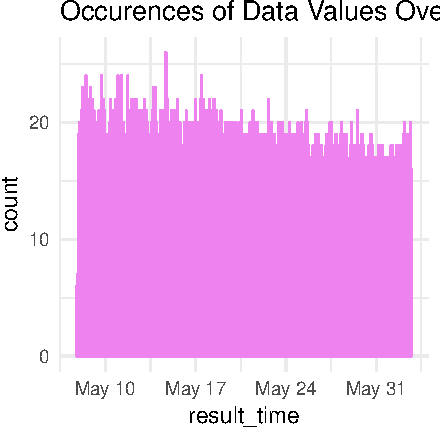
\includegraphics{Project1WriteUp_files/figure-latex/unnamed-chunk-11-1} \end{center}

Humidity and Temperature by time and height

\begin{center}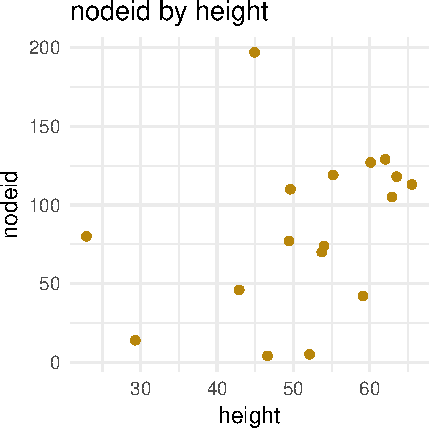
\includegraphics{Project1WriteUp_files/figure-latex/unnamed-chunk-12-1} \end{center}

\begin{center}\includegraphics{Project1WriteUp_files/figure-latex/unnamed-chunk-12-2} \end{center}

\begin{center}\includegraphics{Project1WriteUp_files/figure-latex/unnamed-chunk-12-3} \end{center}

\begin{center}\includegraphics{Project1WriteUp_files/figure-latex/unnamed-chunk-12-4} \end{center}

Reflective PAR over time loosely indicates cycles of daylight, and the
maximum value observed of reflective PAR increases with height.

\begin{center}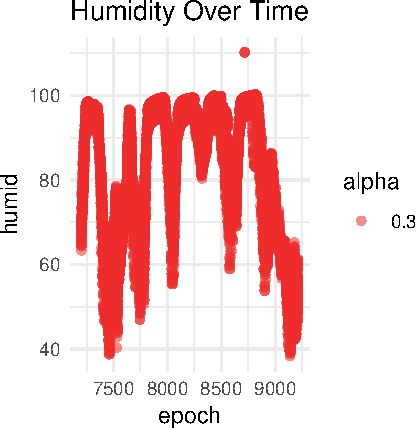
\includegraphics{Project1WriteUp_files/figure-latex/unnamed-chunk-13-1} \end{center}

\begin{center}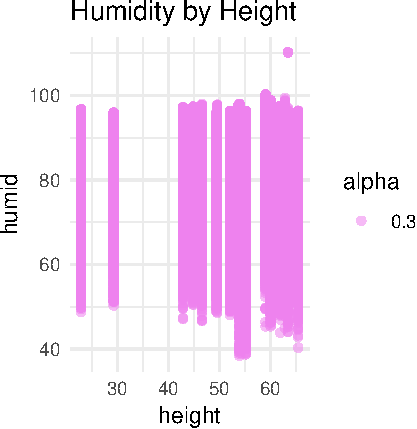
\includegraphics{Project1WriteUp_files/figure-latex/unnamed-chunk-13-2} \end{center}

Are any of the predictors associated with Incident PAR? If so, explain
the relationship.

Incident PAR is visibly cyclical over time. The relationship can be
explained by the daily daylight cycle of the sun rising and setting,
since Incident PAR measures direct sunlight. The second and third plots
here show that certain nodes are exposed to more direct Sunlight, but
not necessarily by height

\begin{center}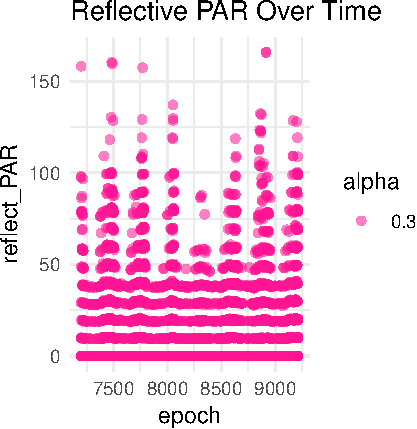
\includegraphics{Project1WriteUp_files/figure-latex/unnamed-chunk-14-1} \end{center}

\begin{center}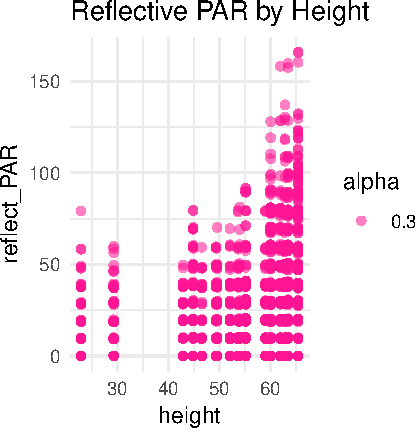
\includegraphics{Project1WriteUp_files/figure-latex/unnamed-chunk-14-2} \end{center}

\begin{center}\includegraphics{Project1WriteUp_files/figure-latex/unnamed-chunk-14-3} \end{center}

*Next, we consider each variable in the context of it's temporal trends,
with height as color cue: ( You can do it for different time scales
during an hour, during a day or during the entire experiment). However,
at least the plots with days as x-axis are required. As shown in the
histogram below, I used epoch as the x variable for time here becuase
their positive, linear relationship justifies our use of epoch as a
standin for time that doesn't lose any information from data\_log. We
could also use result\_time.)

\begin{center}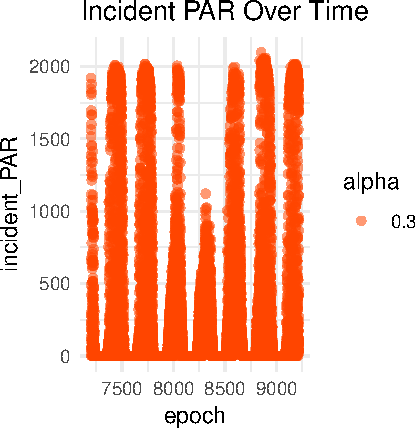
\includegraphics{Project1WriteUp_files/figure-latex/unnamed-chunk-15-1} \end{center}

During the day, incident PAR is noteably least at the lowest height of
the tree. However, there's not a height gradient throughout. Reflective
PAR lacks this trait.

\begin{center}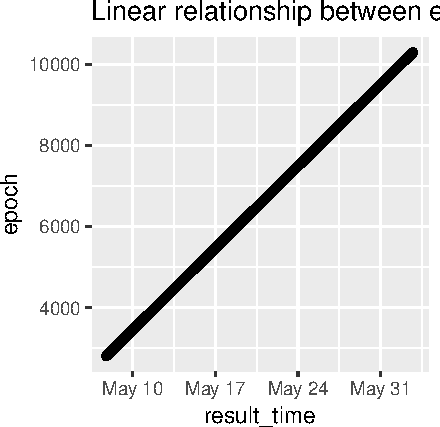
\includegraphics{Project1WriteUp_files/figure-latex/unnamed-chunk-16-1} \end{center}

\begin{center}\includegraphics{Project1WriteUp_files/figure-latex/unnamed-chunk-16-2} \end{center}

The lowest temperatures occur and the least height when and only when
temperature is rising during the day.

\begin{center}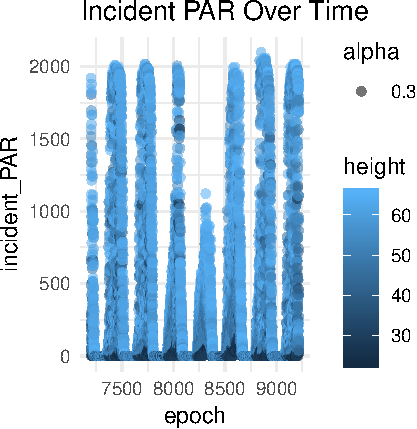
\includegraphics{Project1WriteUp_files/figure-latex/unnamed-chunk-17-1} \end{center}

\begin{center}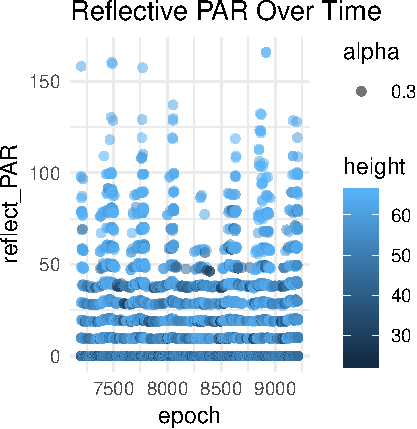
\includegraphics{Project1WriteUp_files/figure-latex/unnamed-chunk-17-2} \end{center}

```

PCA analysis \& scree plot of the data. Can this data be approximated by
some low-dimensional representation?

Describe two/three interesting findings from exploratory analysis of the
data. Try to use the techniques that you have learned, such as
histograms, PCA, K-means, GMM and hierachical clustering etc. Comment on
your interesting findings. Different bonuses are given based on how
interesing your result is.
\textbackslash{}begin\{enumerate\}{[}label=(\alph*){]} \item Finding 1.
2. Finding 2:

Another interesting finding is how little Incident and Reflective
PAR(Direct and Ambien) seem to be correlated when you look at their 2
dimensional scatter plot, given that both measure energy available for
photosynthesis and tell us about drivers for the carbon balance in the
forest.

\begin{center}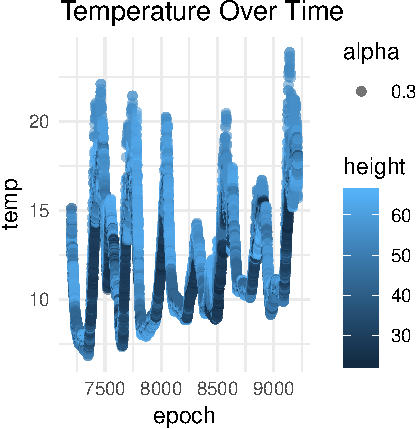
\includegraphics{Project1WriteUp_files/figure-latex/unnamed-chunk-18-1} \end{center}

However, looking at both over time it's clear they experience similar
cycles with the daylight, with the fluctuations of incident PAR having a
much greater magnitude.

\begin{center}\includegraphics{Project1WriteUp_files/figure-latex/unnamed-chunk-19-1} \end{center}

3.(Bonus) Finding 3. Bonus is given only if we also find it interesting.

\section{\texorpdfstring{Graph Critique in the paper (40 pts)\}\\
The overall quality of the paper by Tolle et al. is good. However, some
plots are not perfect from a statistician's point of
view.}{Graph Critique in the paper (40 pts)\} The overall quality of the paper by Tolle et al. is good. However, some plots are not perfect from a statistician's point of view.}}\label{graph-critique-in-the-paper-40-pts-the-overall-quality-of-the-paper-by-tolle-et-al.-is-good.-however-some-plots-are-not-perfect-from-a-statisticians-point-of-view.}

\begin{itemize}
\item
  Figure 3{[}a{]} shows the distributions of sensor readings projected
  onto the value dimension, using a histogram. It turns out that both
  the incident and reflected PAR have long tail. We could not read full
  information from this histogram. Try to make a better plot with log
  transform of the data.
\item
  What message do the boxplots in Figure 3{[}c{]} and 3{[}d{]} try to
  convey? Do you think the plots convey the right messages? If not
  generate a new plot with the same data. Hint: compare to some plots in
  Figure 4. \emph{item Any suggestions for improving the first two plots
  in Figure 4? Can you distinguish all the colors in these two plots?
  }item Comment on Figure 7. Is it possible to generate a better
  visualization to highlight the difference between network and log
  data?
\item
  1: ``10-bit Atmel Microcontroller with 128KBytes In-System
  Programmable Flash''
  \url{http://ww1.microchip.com/downloads/en/DeviceDoc/doc2467.pdf}
\item
  2: ``Analog to Digital Conversion''
  \url{https://learn.sparkfun.com/tutorials/analog-to-digital-conversion/relating-adc-value-to-voltage}
\end{itemize}


\end{document}
